%_____________________________________________________________________________________________
% LATEX Template: Department of Comp/IT BTech Project Reports
% Main Report
% Sun Apr 1 20:40:00 IST 2011
%
%_____________________________________________________________________________________________

\documentclass[a4paper,12pt,onecolumn]{report}
%_____________________________________________________________________________________________
% Inclusion of Required Packages
%_____________________________________________________________________________________________
\usepackage[dvips]{graphics}
\usepackage{color}
\usepackage{epsfig,float}
\usepackage{hyperref}

%_____________________________________________________________________________________________
% Page Layout
%_____________________________________________________________________________________________

 \usepackage[left=2.5cm,top=2cm,right=2cm,bottom=2cm,bindingoffset=0.5cm]{geometry}

%\usepackage{geometry}
%\geometry{a4paper,left=35mm,right=20mm,top=20mm,bottom=20mm}
\setlength{\textwidth}{6.5in}
\setlength{\textheight}{10in}
\setlength{\topmargin}{0.0in}
\setlength{\oddsidemargin}{0.0in}			% Customisable
\setlength{\headheight}{0.0in}
\setlength{\headsep}{0.0in}
\setlength{\topskip}{0.0in}
%_____________________________________________________________________________________________
% Font Definition
%_____________________________________________________________________________________________
\fontencoding{T1}		% Font specification : Times New Roman, Bold, Normal, 18
\fontfamily{cmr}		% Roman
\fontseries{m}			% Medium
\fontshape{n}			% Upright
\fontsize{14pt}{5}
\linespread{1.5}		% Vertical spacing between lines
\selectfont			% Select the specified font

\graphicspath{{./figs/}}

%_____________________________________________________________________________________________
% Main report starts here
%_____________________________________________________________________________________________

\begin{document}	% Start of Report
%_____________________________________________________________________________________________
%\pagestyle{empty}
%_____________________________________________________________________________________________
% Title page: Specifies a custom-made title page
%_____________________________________________________________________________________________
\DeclareGraphicsExtensions{.png, .ps}
\begin{titlepage}
\begin{center}
\LARGE{\bf{USER INTERFACE GENERATION USING MACHINE LEARNING\\}}	% LARGE = 17.28
%\vspace{10pt}
\Large{\bf{A Project Report\\}}		% Large = 14.40
\Large{\em{Submitted by\\}}
\begin{table}[htbp]
	\begin{center}
	\begin{tabular}{ l c c l }
	\Large\bf{Mihir U. Mistry} & & & \Large\bf{111503042} \\[0.3cm]
	\Large\bf{Varad V Ghodake} & & & \Large\bf{111503022} \\[0.3cm]
	\Large\bf{Ameya A. Apte} & & & \Large\bf{111503010} \\
	\end{tabular}
	\end{center}
	\end{table}
\Large{\em{in partial fulfillment for the award of the degree\\ \vspace{1.5pt}of\\}}
\LARGE{\bf{B.Tech Computer Engineering\\}}% Mention only appropriate degree.
%\vspace{10pt}
%names of advisors
\Large{Under the guidance of\\ }
\Large{\bf{Dr. S. B. Mane}\\}
\Large{College of Engineering, Pune\\}
%\vspace{8pt}
%coep logo added
%\begin{figure}[h]
%\centering
%\includegraphics[width=3cm,height=3cm]{coeplogo.eps}
%\end{figure}
\Large{\bf{DEPARTMENT OF COMPUTER ENGINEERING AND \\INFORMATION TECHNOLOGY,\\
COLLEGE OF ENGINEERING, PUNE-5}}
\vfill
\large{May, 2019}
\end{center}
\end{titlepage}

%\maketitle			% *Generate* the defined title. No definition - no gereration

%_____________________________________________________________________________________________
% LATEX Template: Department of Comp/IT BTech Project Reports
% Certificate Page
% Sun Mar 27 10:25:35 IST 2011
%
% Note: UK English spellings used.
%_____________________________________________________________________________________________
\thispagestyle{empty}
\linespread{2}
\begin{center}			% LARGE = 18
	\Large{\bf{DEPARTMENT OF COMPUTER ENGINEERING AND\\  INFORMATION TECHNOLOGY,\\
	       COLLEGE OF ENGINEERING, PUNE\\}}
\end{center}

\vspace{20pt}			% Vertical space between dept name and ``certi''

\begin{center}
	\Large{\bf{CERTIFICATE\\}}
\end{center}

\vspace{20pt}

\linespread{1.5}			% Double spacing between lines
\selectfont
\large{
Certified that this project, titled ``USER INTERFACE GENERATION USING MACHINE LEARNING''
has been successfully completed by \\
\begin{table}[htbp]
	\begin{center}
	\begin{tabular}{ l c c l }
	\Large\bf{Mihir U. Mistry} & & & \Large\bf{111503042} \\ [0.3cm]
	\Large\bf{Varad V. Ghodake} & & & \Large\bf{111503022} \\ [0.3cm]
	\Large\bf{Ameya A. Apte} & & & \Large\bf{111503010} \\
	\end{tabular}
	\end{center}
	\end{table} \\
and is approved for the partial fulfillment of the requirements for the degree of
``B.Tech. Computer Engineering''.
}

\vspace{60pt}

\begin{center}		% Horizontal spacing used to keep the signatures in columns at the ends of
			% lines

SIGNATURE\hspace{\stretch{1}}SIGNATURE\\
\normalsize{\bf{Dr. S. B. Mane\hspace{\stretch{1}}Prof. Vahida Attar\\
Project Guide\hspace{\stretch{1}}Head}\\
Department of Computer Engineering\hspace{\stretch{1}}Department of Computer Engineering\\
and Information Technology,\hspace{\stretch{1}}and Information Technology,\\
College of Engineering Pune,\hspace{\stretch{1}}College of Engineering Pune,\\
Shivajinagar, Pune - 5.\hspace{\stretch{1}}Shivajinagar, Pune - 5.}
\end{center}
		% Certificate page will come here. But its been typeset
				% independently in certi.tex

%_____________________________________________________________________________________________
% LATEX Template: Department of Comp/IT BTech Project Reports
% Abstract of Report
% Sun Mar 27 10:34:00 IST 2011
%_____________________________________________________________________________________________
\newpage
%\begin{abstract}
%\addcontentsline{toc}{chapter}{Abstract}	% This makes sure abstract is included in contents.
\begin{center}
\Large \textbf{Abstract}
\end{center}
Every product development starts with idea conceptualization and design. The ideators’ and designers’ first choice is sketching the idea to conceptualize the product. After a few iterations of product design mockups/prototypes are passed on to developers who have the job to convert these designs into a functional product by grasping the design concepts and using their coding skills. Work stops whenever one discipline finishes a portion of the project and passes responsibility to another discipline. Our service leverages computer vision and machine learning, to automate the typical task of converting mockups to websites and help the developer focus on the minute details of the design. As a proof of concept this project we will be focussing on web mockups but the functionality can be easily extended to mobile applications too.
This service will consist of two stages firstly accepting images of web mockups, hand-drawn sketches and identifying the various HTML components in the sketch using Convolutional Neural Networks and tag them appropriately, secondly, the identified components will be converted to code based on HTML5, Flexbox, React and Bootstrap.
The service will try and bridge the gap between designers and developers by simplifying the product development process and hence offer end to end solution. This will also help people with little or almost no knowledge of web development to bring their design ideas into reality.
 
%\end{abstract}

%_____________________________________________________________________________________________
	% Absract: Independently typeset in file abstract.tex

\thispagestyle{empty}
\tableofcontents		% *Generate* the table of contents. No content - no table
				% LATEX needs to run 2-3 times over source to get this correct

\pagenumbering{roman}	% Lowercase roman numbering for prelim sections
%\listoftables
%\addcontentsline{toc}{chapter}{List of Tables}

\listoffigures
\addcontentsline{toc}{chapter}{List of Figures}

%\chapter*{List of Symbols}
%\addcontentsline{toc}{chapter}{List of Symbols}

\newpage
\pagenumbering{arabic}	% Change to Arabic numbers for main chapters.

%_____________________________________________________________________________________________
% LATEX Template: Department of Comp/IT BTech Project Reports
% Sample Chapter
% Sun Mar 27 10:25:35 IST 2011
%
% Note: Itemization, enumeration and other things not shown. A sample figure is included.
%_____________________________________________________________________________________________

\chapter{Introduction}
Computer vision is a field of computer science that works on enabling computers to see, identify and process images in the same way that human vision does, and then provide appropriate output. It is like imparting human intelligence and instincts to a computer. In reality though, it is a difficult task to enable computers to recognize images of different objects.
Computer vision is closely linked with artificial intelligence, as the computer must interpret what it sees, and then perform appropriate analysis or act accordingly. With the help of computer vision and deep learning the process of website development can be aided to make it more robust,flexible and fast.

\section{The gap between design and development}
%Th is is a section. We can cite a reference like this: \cite{INTERNET} Citation. See references.tex for the entry.
With the technological advancement in the 21st-century, everybody wants to experience the best technology without spending too much of their time and exhausting their busy brains. The same goes for surfing the websites or mobile applications as well where the quick and efficient the website or the mobile application responds, the successful outcomes it obtains. In short, it is about consumers nowadays! And, when it comes to the mobile application or website user satisfaction, most technology firms turn towards the applications’ User Interface (UI) and User Experience Design (UX).
The User Interface (UI), is the process of improving the presentation and the interactivity of the web or mobile application. It focuses on the app’s look and interacts with the users. Each screen, page, buttons and other visual elements you see while using an application is the User Interface of that application.
User Interface Design process involves a lot a creativity that starts on a whiteboard where designers share ideas. Once a design is drawn, and after iterations among the design team, a design mockup is ready. Now, these mockups are passed on to the Development Team. The developers work on to convert these mockups into actual functional units. This is again verified by the design team and a final product is ready after many iterations.
Work stops whenever one discipline finishes a portion of the project and passes responsibility to another discipline. This process takes several iterations and consumes a lot of effort and time. There is a big gap in how the ideas are exchanged between designers and developers. There are ways in which the designer designs an expected view with various drawing tools like Photoshop and CorelDraw. Developers try to mimic these prototypes. But the output of drawing tools is of no help in terms of generating the code for the developer. This shows there is a gap in this process and a big scope of improvement in the whole process of development.

\section{Bridging the gap}
There are various options being tried to bridge the gap. There are drawing software like PhotoShop, CorelDraw which are used by designers to generate the actual design mockups. So that the Development team can try and mimic the exact design submitted by the Design team. But efforts are consumed on both the design side to create the mockups and the development side to mimic them. The purpose of mockups is just to transfer the ideas.
What if we can automate this whole process and try to bridge the gap. An application that takes the photographs of the whiteboard drawings of the Design Team and gives a functional editable code for the developer to work on. This will save time on both ends by removing the idea of creating design mockups on specialised software and developers trying to mimic it.

\section{Role of Computer Vision and ML}
Computer Vision enables developer to leverage existing ‘machine capabilities’ to sense patterns and shapes.the
Computer Vision forms the core of this service. Neural Networks based architectures, such as R-CNN, Fast-RCNN or YOLO built on standard ML libraries like TensorFlow and Keras will help to detect the DOM components user wants in the web page. Detecting DOM elements, unlike common objects, is a comparatively difficult objective; mainly because of the lack of the necessary amount of training data.

	\subsection{Neural Networks}
	Artificial Neural Networks are the biologically inspired simulations performed on the computer to perform certain specific tasks like clustering, classification, pattern recognition etc. Artificial Neural Networks, in general — is a biologically inspired network of artificial neurons configured to perform specific tasks. Neural networks resemble the human brain in the following two ways -

	\begin{itemize}
		\item A neural network acquires knowledge through learning.
		\item A neural network’s knowledge is stored within inter-neuron connection strengths known as synaptic weights.
	\end{itemize}

	\begin{figure}[H]
		\centering
		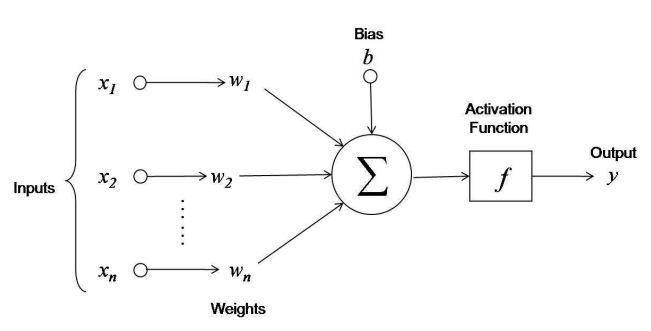
\includegraphics[width=6in]{artificial_neuron}
		\caption
		{Basic structure of an artificial neuron}
	\end{figure}

	Artificial neural networks can be viewed as weighted directed graphs in which artificial neurons are nodes and directed edges with weights are connections between neuron outputs and neuron inputs. The Artificial Neural Network receives input from the external world in the form of pattern and image in vector form. These inputs are mathematically designated by the notation x(n) for n number of inputs. Each input is multiplied by its corresponding weights. Weights are the information used by the neural network to solve a problem. Typically weight represents the strength of the interconnection between neurons inside the neural network.

	\begin{figure}[H]
		\centering
		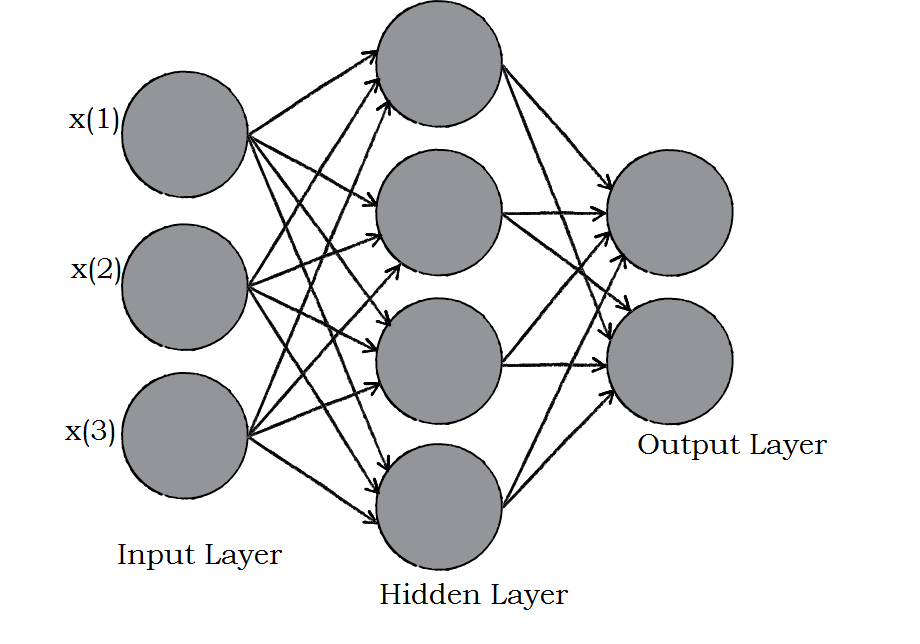
\includegraphics[width=6in]{multilayer_nn}
		\caption
		{Multilayer Neural Network with a hidden layer}
	\end{figure}

	The weighted inputs are all summed up inside computing unit (artificial neuron). In case the weighted sum is zero, bias is added to make the output not- zero or to scale up the system response. Bias has the weight and input always equal to ‘1’. The sum corresponds to any numerical value ranging from 0 to infinity. In order to limit the response to arrive at desired value, the threshold value is set up. For this, the sum is passed through activation function. The activation function is set of the transfer function used to get desired output. There are linear as well as the nonlinear activation function.

	\subsection{Convolutional Neural Network}

	The image is divided into receptive fields that feed into a convolutional layer, which then extracts features from the input image. The next step is pooling, which reduces the dimensionality of the extracted features (through down-sampling) while retaining the most important information (typically through max pooling).
	Another convolution and pooling step is then performed that feeds into a fully connected multilayer perceptron. The final output layer of this network is a set of nodes that identify features of the image (in this case, a node per identified number). You train the network by using back-propagation

	\begin{figure}
		\centering
		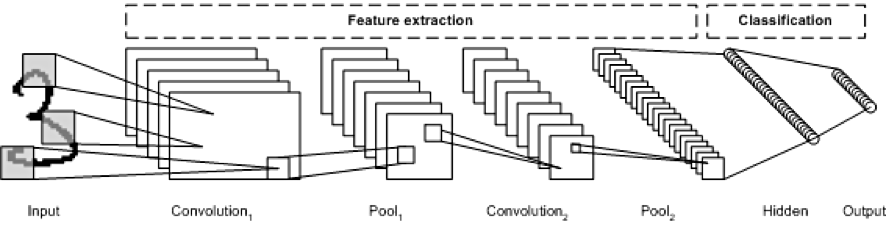
\includegraphics[width=6in]{cnn}
		\caption
		{A Convolutional neural network consisting of multiple steps}
	\end{figure}

	\subsection{RCNN}

	For each image, there is a sliding window to search every position within the image as below. It is a simple solution. However, different objects or even same kind of objects can have different aspect ratios and sizes depending on the object size and distance from the camera. And different image sizes also affect the effective window size. This process will be extremely slow if we use deep learning CNN for image classification at each location.
	In R-CNN the CNN is forced to focus on a single region at a time because that way interference is minimized because it is expected that only a single object of interest will dominate in a given region. The regions in the R-CNN are detected by selective search algorithm followed by resizing so that the regions are of equal size before they are fed to a CNN for classification and bounding box regression.
	Steps:

	\begin{itemize}
		\item NN uses selective search to generate about 2K region proposals, i.e. bounding boxes for image classification.
		\item Then, for each bounding box, image classification is done through CNN.
		\item Finally, each bounding box can be refined using regression.
	\end{itemize}

	\subsection{YOLO (You Only Look Once)}

	Compared to other region proposal classification networks (fast RCNN) which perform detection on various region proposals and thus end up performing prediction multiple times for various regions in a image, Yolo architecture is more like FCNN (fully convolutional neural network) and passes the image (nxn) once through the FCNN and output is (mxm) prediction. This the architecture is splitting the input image in mxm grid and for each grid generation 2 bounding boxes and class probabilities for those bounding boxes. Note that bounding box is more likely to be larger than the grid itself.
	It also makes predictions with a single network evaluation unlike systems like R-CNN which require thousands for a single image. This makes it extremely fast, more than 1000x faster than R-CNN and 100x faster than Fast R-CNN

	\subsection{Optical Character Recognition}

	OCR (optical character recognition) is the recognition of printed or written text characters by a computer. This involves photo scanning of the text character-by-character, analysis of the scanned-in image, and then translation of the character image into character codes, such as ASCII, commonly used in data processing. The current age OCR implementations work with a very superior accuracy for printed english text but the accuracies are lower for handwritten english text. Advancements in OCR have enabled detection of not only printed text but also handwritten content. Multiple cloud services provide APIs for recognition of english handwritten text.


%_____________________________________________________________________________________________
	% Add each chapter here in this fashion.
				% No need to write all font and page specs in the chapter
				% files. There only typesetting tags are required.
%_____________________________________________________________________________________________
% Department of Comp/IT BTech Project Report
%_____________________________________________________________________________________________

\chapter{Literature Review}

  \section{Pix2code}
    Transforming a graphical user interface screenshot created by a designer into computer code is a typical task conducted by a developer in order to build customized software, websites, and mobile applications. In this paper, deep learning methods are  leveraged to train a model end-to-end to automatically generate code from a single input image with over 77% of accuracy for three different platforms (i.e. iOS, Android and web-based technologies).
    The project focuses only on the front end aspect and has little or no consideration of the backend integration required. It aims mobile and web platform underlining the fact that transforming images to component specification files is the important step, the later part of code generation can be made flexible and pluggable. This project was one of the first papers which discussed the approach of using deep learning techniques to generate interfaces based on wireframes.

  \section{Sketch2Code}
    This is a experimental project developed by a team at Microsoft AI Lab the project demonstrates the feasibility of the idea. It also provides datasets for training Neural networks. This project accepts hand drawn mockups as input and generates simple HTML code. The accuracy the project provides is comparatively less, although the image tagging and component file generation is strong.
    Currently this project is published and hosted on azure. Although the results generated are not very accurate and the HTML based alignment of components is inaccurate. Another peculiarity about this project is that it uses neural network as a service based on Microsoft custom vision API. This is a innovative approach to move complex neural networks to the cloud and simplify the process of training and testing.

  \section{Airbnb design team}
    Airbnb design team is working on a project which would convert hand drawn wireframes to React applications. This project is based on a end to end approach and uses Neural networks to both identify elements in the sketch and to convert the structured data of element locations into code. Their aim is to reduce the the development time for airbnb products. The company states this is a experimental project and an ongoing exploration.No source code has been provided as the project is in very early stage. The project shows promising progress a  demo showcase it’s engine working in real time meaning the model is lightweight and proves the potential this idea has. Although the documentation states that the training set is limited and needs improvement for improved results on varied data sets

  \section{Deepcoder}
    This is a very noteworthy paper published in 2017, the paper discusses the possibility of computers writing code themselves  using complex deep neural networks. The system accepts large datasets of source codes from the internet and trains neural networks based on these datasets. It focusses at Domain Specific Languages, The neural net predicts the probability of occurrence of a higher level function in the code, based on these probabilities and with the help of various search techniques the  neural net produces code based in the DSL
    Although this project is not directly related to our idea it forms the basis of the concept of producing deployable code based on deep learning techniques and high computation. Multiple research publication cite this paper in the field of computer vision as it is considered as  a cornerstone. This project fueled the concept of generating code using code based on vision, imagery, structured data and even other source codes.




%_____________________________________________________________________________________________

%_____________________________________________________________________________________________
% Department of Comp/IT BTech Project Report
%_____________________________________________________________________________________________

\chapter{System specifications}

  \section{Objectives}
    \begin{itemize}
      \item Pre processing input image
      \item Detection Regions of Interest (basic HTML elements) in the image
      \item Labelling these regions using machine learning
      \item Generating code based on component files
  	\end{itemize}
  \section{Operating environment}
    \begin{itemize}
      \item A hosted machine with >8GB RAM for processing images and gathering results
      \item Graphical processing focussed machines for training the models
      \item Camera with >8MP image quality for capturing wireframes
    \end{itemize}
  \section{Libraries/Dependencies}
    \begin{itemize}
      \item Tensorflow framework
      \item Keras
      \item Python 3.0
      \item OpenCV
      \item Tesseract OCR
    \end{itemize}
  \section{Online services}
    \begin{itemize}
      \item Amazon Web Services (Hosting services)
      \item Google OCR Engine
      \item Github (Version Control)
    \end{itemize}



%_____________________________________________________________________________________________

%_____________________________________________________________________________________________
% Department of Comp/IT BTech Project Report
%_____________________________________________________________________________________________

\chapter{System Design}

  \section{Architecture overview}
  A multi-step process will be followed to convert the images provided by the user into a functional code. The process is broadly divided into two steps:
  \begin{itemize}
		\item Processing images to detect and label ROI and storing in  a structured format.
    \item Conversion of structured specification of ROI into target code.
	\end{itemize}
  Initially a different approach was experimented which was a single step process. This was heavily relying on the neural networks’ training and accuracy. But it was observed that the dataset available for training was not adequate and using such a complex neural network was an overkill as the problem at hand can be categorized as a image classification problem. Hence an improved architecture was used to implement the solution
  \begin{figure}
		\centering
		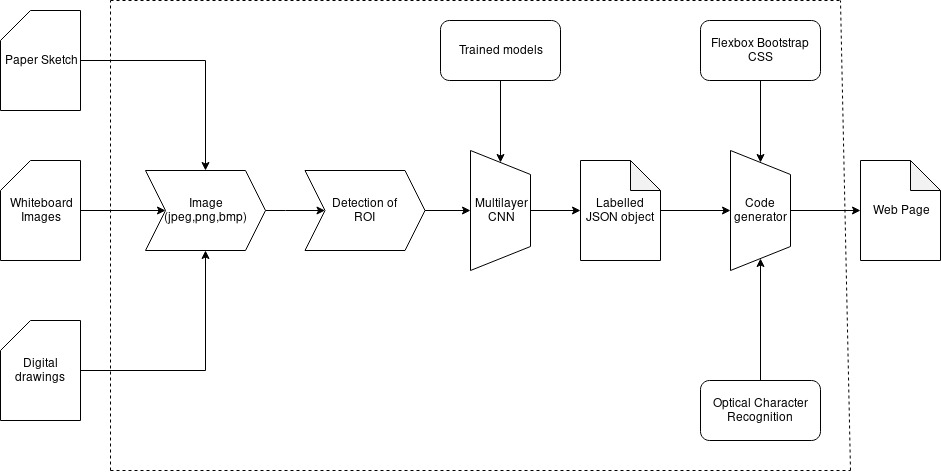
\includegraphics[width=6in]{architecture}
		\caption
		{A block diagram of the complete process}
	\end{figure}

  \section{Vision Model}
    An integral part of our solution is to understand the mock up sketch image the user provides. We need a solution to detect the regions of interests (ROIs) from the user provided hand drawn sketch, identify the DOM element corresponding to the drawing, and detect handwritten texts within the sketch. The advancements in image processing and computer vision provides many possible methods to do the same. We have different classification and detection model architectures available to work with which are proven to give better results. Also some image preprocessing and dataset augmentation methods can boost the results of these models. We will discuss the experiments performed and the method we used for our solution.

    \subsection{Experiments with Object Detection Algorithms}
      Object Detection Algorithms are different from classification algorithms. The difference between object detection algorithms and classification algorithms is that in detection algorithms, we try to draw a bounding box around the object of interest to locate it within the image. Unlike image classification, this problem cannot be solved by building a standard convolutional network followed by a fully connected layer. The reason being that the output layer here is not constant and variable in size, because the image can have variable number of occurence of objects in an image. Therefore, a different set of algorithms like R-CNN [8], Faster-RCNN [9] and YOLO [10] are used which are helpful in solving the problem of finding and classifying design layout elements[1]. These networks are capable of finding the ROIs as well as classifying them into classes.

    \subsection{RCNN}
      The RCNN uses selective search to find out the region proposals. Using this algorithm around 2000 regions are detected. The regions are of various sizes and aspect ratio spread over the image depending on the image features and contours defined in the selective search algorithm. These proposed regions are then passed to a Convolutional Neural Network for classification and elimination.
      Selective search combined with a simple CNN was used to implement this method. The CNN classification accuracy was around 81%. But the main challenge was elimination of hierarchical regions (regions inside regions). Therefore many regions were detected in a same image.
      The speed of RCNN is slow and was difficult to use it for a real time application. Moreover the model trained on the available training data generated a lot of false ROIs and gave poor results. With the help of more diverse training a data a better model could have been trained. But however the speed of RCNN is always an issue for real time implementation.

    \subsection{YOLO (You Only Look Once)}
      YOLO as the name suggests looks at the image only once. In this architecture there is no separate model for region proposals. The output of the network is regions along with its class. It also makes predictions with a single network evaluation unlike systems like R-CNN which require thousands for a single image. This makes it extremely fast, more than 1000x faster than R-CNN and 100x faster than Fast R-CNN.
      YOLO and such models require a large training dataset and are very particular and fitting our dataset to this model was difficult. It was difficult to find a configuration for which the model was at least able to overfit on the dataset. The difficulty in finding the configuration and very less dataset even to overfit was the reason further experiment on this model was stopped.

    \subsection{Faster-RCNN}
      Selective search is a slow and time-consuming process affecting the performance of the network. Therefore, Faster RCNN uses an object detection algorithm that eliminates the selective search algorithm and lets the network learn the region proposals. These networks are called Region Proposals Networks (RPNs). The image is provided as an input to a convolutional network which provides a convolutional feature map. The predicted region proposals are then reshaped using a RoI pooling layer which is then used to classify the image within the proposed region and predict the offset values for the bounding boxes.
      Faster-RCNN model proved better than both RCNN and YOLO. The classification accuracy was around 82% but it was short on finding all the ROIs. The RPN loss was unable to decrease after a certain point. As a result not all the ROIs were detected in an image; which is a major drawback in our application. It leads to missing out some DOM elements. Better results through separate detection and classification method and unavailability of big and diverse dataset held us from experimenting further with this network.

    \subsection{Conclusion}
      The above models were tried to train on a dataset containing of around 100 labelled images. With the experiments performed to train these complex algorithms; it was clearly observed that more training data and diverse data was required.
      Some data augmentation techniques like binarizing the image, changing color values and changing contrast values were applied on the available images. Other augmentation techniques like flipping and rotating the images were not applicable for the problem set.
      The techniques did not increase the dataset significantly and the only option seemed to be creating more hand-drawn design layout images and manually labelling all the DOM elements in it.

  \section{Modified Approach}
    The input image provided by the user is usually of two colors : the ink and the background colors. These high contrast of colors can be used to detect regions first and then later classify them. Also the above models performed poorly on the ROI detection phase and not the classification phase. The image pre-processing can be done using tools like OpenCV to get the desired regions.
    The results conspicuously hinted towards another approach by finding the Regions and Interests first, rather than Object Detection over the whole image, and then using modified deep learning algorithms to identify the DOM elements.
    So the task of vision model was split into three sections:
    \begin{enumerate}
  		\item Detection of ROIs
      \item Classification of ROIs
      \item Handwriting Recognition
  	\end{enumerate}

    \subsection{Detection of ROI}
      The image captured by the user consists mainly of the white background of the paper and the black/blue sketch drawn on it. Before the various elements of the sketch can be detected it is necessary to figure out multiple regions of interest which can be then passed to a neural network for identification based on a confidence value. The above mentioned property of the input images can be extremely helpful for preprocessing the images.We have used the python interface for OpenCV for processing the images[6] and generating multiple bounding rectangle around the region of interest.

      \subsubsection{Grayscale conversion}
        The input image is a full color image,as the elements of interest have a binary color schema a simple linear transform is used to convert the RGB images to Grayscale (0-255). This helps reduce the dimensionality of the input image with almost no loss as all the information of the sketch is captured in the grayscale image.
%        RGB to Gray: Y = 0.299⋅R+0.587⋅G+0.114⋅B%

        \begin{figure}[H]
      		\centering
      		
\includegraphics[width=6in]{grayscale.jpg}
      		\caption
      		{Output after grayscale transformation}
      	\end{figure}

      \subsubsection{Adaptive thresholding}
        Further the grayscale image can be reduced to binary image, this helps enhance the strokes of the characters and the figures drawn by the user and eliminates all the fine noise[5] in and around the image. A mean value of pixels in a kernel are calculated this is the threshold value of the kernel, a constant value is subtracted from this and the result is compared with the cutoff number, this generated a binary output which is used to binarize the image. The dimensions of the kernel are 7x7 and a very low cutoff value ~10 is used as the major component of the image is close to white i.e the color of the paper. An inverted binary output is generated.
        \begin{figure}[H]
      		\centering
      		
\includegraphics[width=6in]{adaptive.jpg}
      		\caption
      		{Output after adaptive thresholding transformation}
      	\end{figure}

      \subsubsection{Dilation}
        The image is further dilated iteratively to group the nearby elements in order to avoid fragmented region detection.Dilation is a morphological operation which reduces noise and helps join disparate elements in the image. The primary goal of this step is to merge the nearby contours and hence generate bigger, less fragmented regions. A rectangular kernel is used for dilation as the natural structure of most sketches generated by humans are horizontal in nature. Eg. Words, Letters, Textboxes. Based on the size and the shape of the kernel we can generate regions which are horizontal or vertical merging of the fragmented contours. The iteration count, dimensions and shape of the kernel can be varied to generate different regions of interest.
        \begin{figure}[H]
      		\centering
      		
\includegraphics[width=6in]{dilation.jpg}
      		\caption
      		{Output after dilation transform}
      	\end{figure}

      \subsubsection{Finding bounding rectangles}
        Multiple contours are detected in the dilated images. The contours are filtered based on the area and the dimensions of the contour to weed out possible regions which are very small or thin compared to the dimensions of the image. Bounding rectangles are created around the contours in order to mark the regions of interest. These bounding boxes can now be used to crop the regions of interest which can be passed to the Convolutional Neural Network for labelling. The predictions with the highest confidence score can be used for generating codes.
        \begin{figure}[H]
      		\centering
      		
\includegraphics[width=6in]{contour.jpg}
      		\caption
      		{Output after detection of bounding rectangles around regions of interest}
      	\end{figure}

    \subsection{Classification of ROIs}
      Convolutional Neural Networks are widely being used for image classification problems. We used CNN to learn a model by mapping input images to fixed size output vector representing various DOM elements like textbox, radiobutton, checkboxes, labels etc. Now that the Regions of Interests are detected in the previous step they need to be classified into DOM elements. Also there exist some additional falsely detected regions. Such regions need to be discarded.
      \begin{figure}[H]
        \centering
        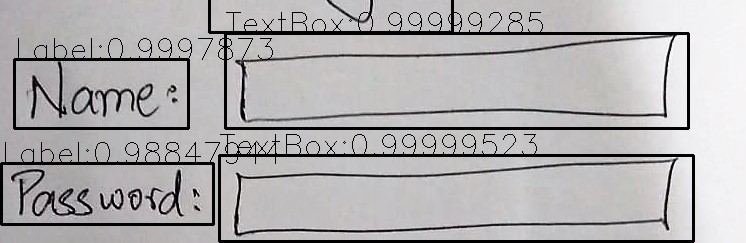
\includegraphics[width=6in]{labelling1.jpg}
        \caption
        {Output after detection of bounding rectangles around regions of interest}
      \end{figure}

      \begin{figure}[H]
        \centering
        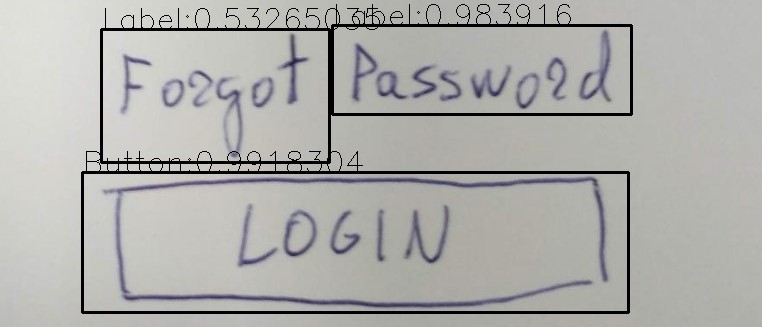
\includegraphics[width=6in]{labelling2.jpg}
        \caption
        {Output after detection of bounding rectangles around regions of interest}
      \end{figure}

      As a part of preprocessing the detected regions were resized into 150x150 images (not maintaining the aspect ratios) and were made grayscale. This input matrix is then passed through two convolution layer and two fully connected layer. The network was kept simple as smaller dataset was available and the problem was simpler. The architecture is shown below:

      \begin{figure}[H]
        \centering
        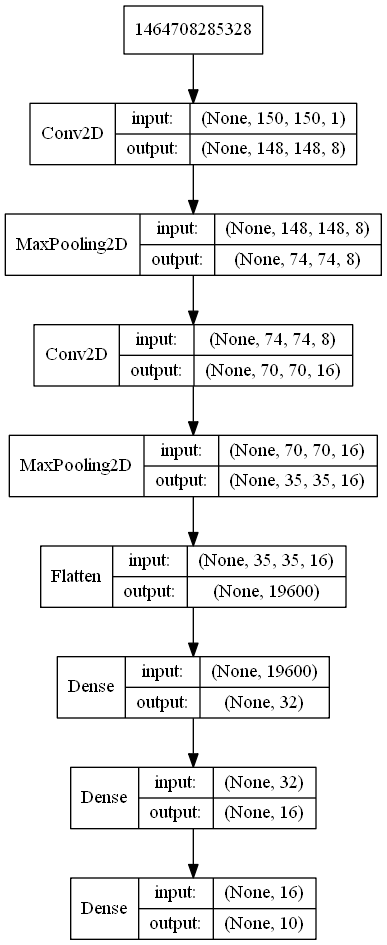
\includegraphics[width=4in]{model}
        \caption
        {Output after detection of bounding rectangles around regions of interest}
      \end{figure}

      A threshold on the confidence score was set. This helped to discard the falsely identified regions as they did not clear the set threshold.
      The model gave a validation accuracy of around 84% after training it for 75 epochs. The less accuracy was majorly due to confusion between radio buttons, check boxes, labels and headings. There is not much visual dissimilarity between them. There is still scope to increase the accuracy of this model by further experimentation.

      \subsection{ Handwriting Recognition}
        There are many cases where the text is written inside the design components. Some examples are hints in textbox, labels, checkboxes, paragraphs. These texts will be handwritten and need to be recognised accurately.

        \begin{figure}[H]
          \centering
          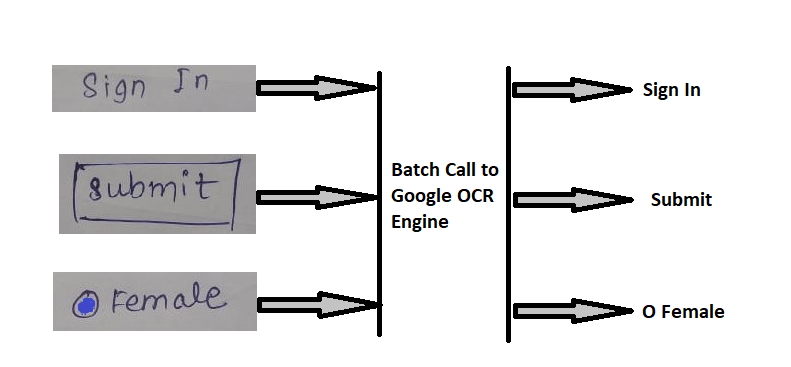
\includegraphics[width=6in]{ocr}
          \caption
          {Output after detection of bounding rectangles around regions of interest}
        \end{figure}

        Each detected design component from the above step was passed to this Text Recognition model to extract the handwritten content. This text will be then associated with the detected component for further steps. Google Optical Character Recognition engine is used as it provides highest handwritten text recognition accuracy. It also provides batch recognition which helps reduce networking delays and cut short the overall processing time.
        The recognised texts are appended to the classification results and saved in a JSON file. This file can be then processed to generate markup language.

      \section{HTML generator}
      The results of the Neural networks are stored in a structured JSON file. Optical character recognition is performed for components containing text. The JSON object generated is a generic object which can be used for generating web elements based on different technologies.The Web engine converts the JSON formatted document layout file into Markup Language Code by detecting the DOM structure based on the coordinates of the regions and their height/width. To represent document layout in JSON, relative position of the element as well as its dimensions are calculated.
      The format of an example DOM element in the JSON file is the following:
      \begin{verbatim}
      {
          "id": "b5e7d988cfdb78bc3be1a9c221a8f744",
          "type": "textbox",
          "height":"100",
          "width":"100",
          "x":"500",
          "y":"400",
         “value”:”Type here”
          "parent": "60c0b53095f81a7bf551b30c93fd20dd",
          "child": “”
      }
      \end{verbatim}
      Modern Browsers support ‘flex-container’ CSS class. This class has some useful built-in features to make web development easier. Vertical and horizontal stacking of elements can be done by just toggling the value of ‘flex-direction’ attribute of this class.
      Besides all the dimension and type related information about the nodes, document metadata also stored in the JSON (eg. Height, Width). Dependant information is calculated geometrically. Orientation and layout [7] of the tags of the HTML document is decided from document height and width values available in the metadata and corresponding changes are reflected in the flexbox orientation. Web engine converts this document layout JSON into code.

      \section{End to End Experience}
        A web service based on MEAN stack was developed to provide a polished end to end solutions for users to consume the service. Users can upload the images for sketch drawn and the service will process the uploaded image using our custom trained tensorflow model on the server and process the results via the web engine and generate HTML code for the user. The structured JSON file along with the bootstrapped HTML code will be available for download as a compressed object.






%_____________________________________________________________________________________________

%_____________________________________________________________________________________________
% Department of Comp/IT BTech Project Report
%_____________________________________________________________________________________________

\chapter{References}
\begin{verbatim}
[1] https://www.ailab.microsoft.com/experiments/30c61484-d081-4072-99d6-e132d362b99d
[2] https://arxiv.org/pdf/1705.07962.pdf
[3] https://airbnb.design/sketching-interfaces/
[4] https://github.com/Microsoft/ailab/tree/master/Sketch2Code
[5]https://medium.com/@ageitgey/machine-learning-is-fun-part-3-deep-learning-and-convolutional-neural-networks-f40359318721
[6]https://towardsdatascience.com/r-cnn-fast-r-cnn-faster-r-cnn-yolo-object-detection-algorithms-36d53571365e
[7] https://arxiv.org/pdf/1504.08083.pdf
[8] https://arxiv.org/pdf/1311.2524.pdf
[9] https://arxiv.org/pdf/1506.01497.pdf
\end{verbatim}






%_____________________________________________________________________________________________


%_____________________________________________________________________________________________
\end{document}			% End of Report
